\documentclass[a4paper,11pt]{jarticle}
%\documentclass[twoside]{jbook}
%\documentclass[twoside]{jreport}

\usepackage[dvipdfmx]{hyperref}

% Page & text layout
\usepackage{geometry}
\geometry{%
  a4paper,%
  top=2.5cm,%
  bottom=2.5cm,%
  left=2.5cm,%
  right=2.5cm%
}
\tolerance=750
\hfuzz=15pt
\hbadness=750
\setlength{\emergencystretch}{15pt}
\setlength{\parindent}{0cm}
\setlength{\parskip}{0.2cm}
\makeatletter

\renewcommand{\paragraph}{%
  \@startsection{paragraph}{4}{0ex}{-1.0ex}{1.0ex}{%
    \normalfont\normalsize\bfseries\SS@parafont%
  }%
}
\renewcommand{\subparagraph}{%
  \@startsection{subparagraph}{5}{0ex}{-1.0ex}{1.0ex}{%
    \normalfont\normalsize\bfseries\SS@subparafont%
  }%
}
\makeatother

\usepackage{fancyhdr}
\pagestyle{fancyplain}
\fancyhead[LE]{\fancyplain{}{\bfseries\thepage}}
\fancyhead[CE]{\fancyplain{}{}}
\fancyhead[RE]{\fancyplain{}{\bfseries\leftmark}}
\fancyhead[LO]{\fancyplain{}{\bfseries\rightmark}}
\fancyhead[CO]{\fancyplain{}{}}
\fancyhead[RO]{\fancyplain{}{\bfseries\thepage}}
\fancyfoot[LE]{\fancyplain{}{}}
\fancyfoot[CE]{\fancyplain{}{}}
\fancyfoot[RE]{\fancyplain{}{\bfseries\scriptsize}}
\fancyfoot[LO]{\fancyplain{}{\bfseries\scriptsize}}
\fancyfoot[CO]{\fancyplain{}{}}
\fancyfoot[RO]{\fancyplain{}{}}

\usepackage{graphicx}


\begin{document}

\begin{titlepage}
\vspace*{7cm}
\begin{center}%
{\LARGE \bf 次世代ものつくりプラットフォーム(HPC/PF)\\

PDI(パラメータ空間設計・入力支援)サブシステム\\

操作説明書\\}
\vspace*{2.5cm}
\bf Version 1.4.2\\
\vspace*{3.5cm}
%{\large\bf (株)富士通システムズ・イースト\\}
\vspace*{1cm}
%{\large\bf 解析ソリューション部\\}
\vspace*{2cm}
\bf 2015年9月\\
\end{center}
\end{titlepage}


\newpage

{\Large\bf 改版履歴}

\vspace{12pt}
\begin{tabular}{|l|l|l|} \hline
リリース & 版数 & 備考\hspace*{11cm}\\ \hline
2013/02 & 1.0 & 初版\\ \hline
2013/06 & 1.1 & 「{\tt $--$no\_all}」オプションの追加\\
 & & {\tt <cond>ノードの比較演算子の変更}\\ \hline
2014/03 & 1.2 & templateファイル記述方式変更\\
 & & {\tt 対応ソルバの追加}\\ \hline
2014/10 & 1.3 & ワークフローのLua化に対応\\ \hline
2014/10 & 1.3.1 & スナップショットファイル名を{\tt .pdi\_params}から{\tt snap\_params.pdi}に変更\\ \hline
2015/08 & 1.4 & JAXAの多目的進化計算(MOEA)に対応\\ \hline
2015/09 & 1.4.1 & JAXAの多目的進化計算(MOEA)をWindows環境に対応\\
 & & Windows環境用にpy2exeのsetup.pyを提供\\ \hline
2015/09 & 1.4.2 & プリファレンスファイルが存在しない場合にデフォルト設定を使用\\ \hline
\end{tabular}

\newpage
\tableofcontents


\newpage
\section*{はじめに}

本書は、HPC/PF システムの PDI サブシステムについての操作説明書です。


HPC/PFシステムは、数値解析シミュレータとその周辺処理ツール群であり、HPC/PFシステムを構成するサブシステムの1つであるPDIは、ユーザのパラメータ空間設計およびパラメータ入力を支援します。


本書では、PDIのインストール方法および操作方法について説明します。

\newpage
\section{インストール}

\vspace{12pt}
PDIのインストール方法について説明します。

\subsection{動作環境}

想定される動作環境を以下に示します。

表2-1 PDI動作環境

\begin{tabular}{|l|l|}
\hline
アーキテクチャ & AMD64, IA32\\ \hline
OS & Linux 2.6/3.x\\
   & MacOS 10.9/10.10\\
   & Windows 7/8\\ \hline
ソフトウエア & Python 2.x\\
             & wxPython 2.7以降/3.0\\ \hline
\end{tabular}

\subsection{必須ソフトウエアのインストール}

\subsubsection{Pythonのインストール}

\textbf{(1) Linux}

多くのLinuxディストリビューションでは、Pythonの実行環境はOSに含まれています。ログイン後にターミナルで「{\tt which python}」と入力し、Pythonの実行パスが表示されれば、そのシステムでPythonは使用可能です。

Pythonがインストールされていない場合、各Linuxのディストリビューション管理システムを使用してPythonをインストールすることが可能です。以下に例を示します。

\begin{description}
\item[RedHat/CentOS系] {\ } \\
{\tt sudo yum install python} \\
\item[Debian/Ubuntu系] {\ } \\
{\tt sudo apt-get install python}\\
\end{description}
{\ }\\


\textbf{(2) MacOS}

MacOS環境向けには、Pythonのインストーラパッケージが用意されています。

以下に示すURLより、PDIを動作させる環境にあったインストーラをダウンロードし、実行することでインストールをおこなってください。
\begin{quote}
{\tt http://www.python.org/download/}
\end{quote}
尚、同URLにはPython 3.xのインストーラパッケージも登録されていますが、PDIはPython
3.xでの動作は保証していません。Python 2.xのインストーラパッケージを使用してください。
{\ }\\


\textbf{(3) Windows}

Windows環境向けには、Python 2.7.xのインストーラパッケージが用意されています。

以下に示すURLより、PDIを動作させる環境にあったインストーラをダウンロードし、実行することでインストールをおこなってください。
\begin{quote}
{\tt http://www.python.org/download/}
\end{quote}
尚、同URLにはPython 3.xのインストーラパッケージも登録されていますが、PDIはPython
3.xでの動作は保証していません。Python 2.xのインストーラパッケージを使用してください。

インストーラ実行時に、「Customize Python 2.7.x」という画面が表示され、ここでインストールするPythonの構成を選択する事が出来ます。

\begin{center}
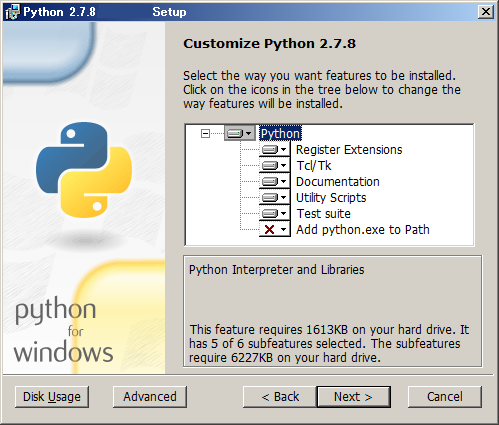
\includegraphics[width=250pt, bb=0 0 499 425]{figs/fig000.png}

図1 Python Windowsインストーラ画面
\end{center}

ここで、デフォルトでは「Add python.exe to Path」という項目が「×」(インストールしない)になっているので、これを「Will be installed on local hard drive」に変更した上でインストールを進めてください。
{\ }\\


\subsubsection{wxPythonのインストール}

\textbf{(1) Linux}

多くのLinuxディストリビューションでは、ディストリビューション管理システムを使用してwxPythonをインストールすることが可能です。以下に例を示します。

\begin{description}
\item[RedHat/CentOS系] {\ }\\
{\tt sudo yum install wxPython}\\
\item[Debian/Ubuntu系] {\ }\\
{\tt sudo apt-get install python-wxgtk2.8}
\end{description}
{\ }\\


\textbf{(2) MacOS}

MacOS環境向けには、wxPythonのインストーラパッケージが用意されています。
以下に示すURLより、PDIを動作させる環境にあったインストーラをダウンロードし、実行することでインストールを行ってください。
\begin{quote}
{\tt http://www.wxpython.org/download.php\#stable}
\end{quote}
{\ }\\


\textbf{(3) Windows}

Windows環境向けには、wxPythonのインストーラパッケージが用意されています。
以下に示すURLより、PDIを動作させる環境にあったインストーラをダウンロードし、実行することでインストールをおこなってください。
\begin{quote}
{\tt http://www.wxpython.org/download.php\#stable}
\end{quote}
{\ }\\



\subsection{PDIのインストール}

PDIのパッケージは、システムの任意の場所に置くことができます。

PDIのディストリビューションに含まれる{\tt pdi\_{\it version}.tar.gz}または{\tt pdi\_{\it version}.zip}ファイル({\tt\it version}は実際の文字列に置き換えてください)を任意のディレクトリに展開します。

{\tt tar.gz}の場合は、tarコマンドで以下のように実行します。

\begin{quote}
{\tt tar xvfz  pdi\_\textit{version}.tar.gz}
\end{quote}


展開を実行すると、以下に示すようなディレクトリ階層が作成されます。

\begin{quote}
\begin{verbatim}
pdi
├── bin
│   ├── pdi
│   └── pdi.bat
├── doc
│   ├── pdi_ug.pdf
│   └── pdi.txt
├── lib
│   └── python
└── conf
     ├── PDI.conf
     └── PDI_log.conf
\end{verbatim}
\end{quote}

PDIの実行コマンドは、{\tt pdi/bin/pdi}(Linux, MacOS)または{\tt pdi/bin/pdi.bat}(Windows)です。

\newpage
\section{操作方法}

PDIの操作方法について説明します。

\subsection{プログラムの起動}

PDIの実行コマンドファイルは、以下のパスに存在します。

\begin{quote}
{\tt (PDIインストールディレクトリ)/pdi/bin/pdi(.bat)}
\end{quote}

PDIを起動する際の、コマンドライン指定の形式を以下に示します。。

\begin{description}
\item[GUIモード] {\ }
\begin{verbatim}
pdi  [-x case_directory] [-d param_desc] [-o output_pattern]
     [-t template_file -t template_file ...] [--no_all]
     [-p param_name:param_value  -p param_name:param_value ...]
\end{verbatim}

\item[バッチモード] {\ }
\begin{verbatim}
pdi {-b | -B} [-x case_directory] [-d param_desc] [-o output_pattern]
    [-t template_file -t template_file ...]
    [-p param_name:param_value -p  param_name:param_value ...]
\end{verbatim}

\item[引数説明] {\ }
\begin{description}
\item[{\tt -b}] {\ }\\
バッチモード実行。
指定された場合、GUIウインドウを表示せず、バッチモードで実行します。
\item[{\tt -B}] {\ }\\
バッチモード実行。
{\tt -b}指定の場合と同じですが、ワークフロー実行用スクリプトファイル({\tt pdi\_generated.lua})の生成は行いません。
\item[{\tt -x  case\_directory}] {\ }\\
ケースディレクトリ指定。
指定されると、PDIは起動時にcase\_directoryにカレントワーキングディレクトリを移動します。指定が省略された場合は、起動ディレクトリとなります。

\item[{\tt -d  param\_desc}] {\ }\\
パラメータ記述XMLファイルの指定。
パラメータ記述XMLファイルのパスを指定します。絶対パスか、カレントワーキングディレクトリからの相対パスで指定します。

\item[{\tt $--$no\_all}] {\ }\\ 
GUIモードにおいて「\_All\_」ページを作成しません。
ただし、パラメータ記述ファイル中に{\tt <group>}タグが一つも存在しない場合は
作成します。

\item[{\tt -t  template\_file}] {\ }\\
ソルバ入力パラメータテンプレートファイルの指定。
入力パラメータテンプレートファイルのパスを指定します。絶対パスか、カレントワーキングディレクトリからの相対パスで指定します。複数指定が可能です。

\item[{\tt -o  output\_pattern}] {\ }\\
出力先ディレクトリ・ファイル名のパターン指定。
サブケース毎に生成する作業ディレクトリ及び作業ディレクトリ配下の入力パラメータファイルのパターンを指定します。パターンは、以下に示す形式で指定します。
\begin{quote}
{\tt directoryname/filename}
\end{quote}
作業ディレクトリ名と配下のファイル名は「/」で区切られます。パターン中に「/」が現れない場合、すべてfilenameと解釈され、カレントワーキングディレクトリ直下にfilenameのパターンで入力パラメータファイルが作成されます。

directorynameが指定された場合、カレントワーキングディレクトリ配下に作業ディレクトリとしてdirectorynameが作成され、その配下にfilenameが作成されます。

directoryname中に「\%P」が含まれている場合、この部分はスイープされるパラメータ値の組み合わせ文字列に置き換えられます。また、「\%Q」がが含まれている場合、この部分はスイープされるパラメータ名+パラメータ値の組み合わせ文字列に置き換えられます。
\begin{quote}
\begin{verbatim}
(例)
ptest%P/PARAMS ⇒ ptest_100_10/PARAMS
ptest%Q/PARAMS ⇒ ptest_Re100_CX10/PARAMS
\end{verbatim}
\end{quote}

パラメータスイープが行われない場合は、「\%P」「\%Q」は空文字列に置き換えられます。
\begin{quote}
{\tt (例) ptest\%P/PARAMS ⇒ ptest/PARAMS}
\end{quote}

filename中に「\%T」が含まれている場合、この部分はtemplate\_fileのベース名に置き換えられます。また、filename中に「\#T」が含まれている場合、この部分はtemplate\_fileの番号に置き換えられます(template\_fileが1個だけ指定されている場合は「\_0」)。

filename中に「\#S」が含まれている場合、この部分は単一ディレクトリ内のサブケース番号(1ディレクトリにつき1サブケースの場合は、常に0)に置き換えられます。

directorynameおよびfilename中に「\#D」、「\#J」が含まれている場合、この部分はそれぞれディレクトリ通番、サブケース通番に置き換えられます。
\begin{quote}
{\tt (例) ptest\#D/PARAMS\#J ⇒ ptest\_0/PARAMS\_0}
\end{quote}

\item[{\tt -p param\_name:param\_value}] {\ }\\
パラメータ値の直接指定。
パラメータ名とパラメータ値のペアを、コマンドラインから直接指定します。複数指定が可能です。パラメータ名とパラメータ値は「:」で区切って記述します。

パラメータ値は、以下のいずれかの形式で指定を行います。
\begin{itemize}
\item 直接指定
\item 範囲、刻み幅指定: 最小値/最大値/刻み幅\\
最小値、最大値、刻み幅を「/」で区切って記述。空白を入れてはならない。
\item 列挙: 値1,値2,...\\
列挙する値を「,」で区切って記述。空白を入れてはならない。
\end{itemize}

尚、直接指定または列挙で文字列値を指定する場合、空白または区切り文字が含まれる場合は「{\tt "}」で囲って指定します。

\end{description}
\end{description}

PDIをGUIモードで実行すると、PDIのメインウインドウが表示されます。

\begin{center}
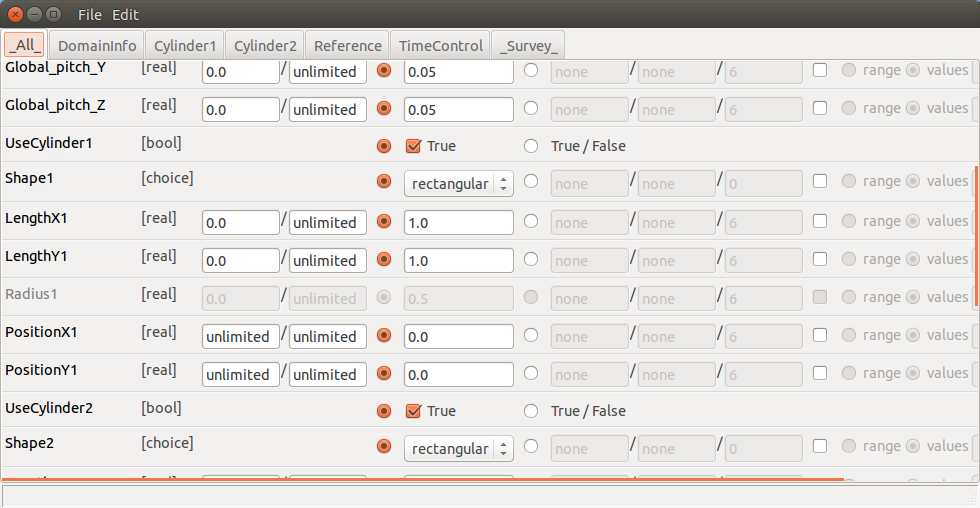
\includegraphics[width=360pt, bb=0 0 982 512]{figs/fig001.png}

図2 PDIメインウインドウ
\end{center}


尚、PDIの終了は、メインウインドウのFileメニューからQuitを選択するか、メインウインドウを閉じることで行えます(MacOSの場合、Quitはメニューバーの「Python」メニューの「{\tt Quit Python}」です)。


\subsection{パラメータ空間設計支援機能}

PDIのパラメータ空間設計支援は、パラメータ定義ファイルの記述に基づいて行われます。

パラメータ定義ファイルは、PDIで設定可能なソルバのパラメータの名前、型、値域、デフォルト値、所属グループなどを記述したXML形式のファイルで、PDIの起動時に「-d」オプションで指定する他、GUIモードの場合は「File」メニューの「{\tt load parameter description file}」からファイルを指定し、ロードさせることができます。


パラメータ定義ファイルがロードされると、GUIモードの場合パラメータ定義ファイル中に記述された各パラメータ項目は、所属するグループごとにタブページにまとめられ、リスト形式で表示されます。所属グループ属性のないパラメータ項目を含めすべてのパラメータ項目は、「ALL」のタブページにまとめられます。


各パラメータ項目は、パラメータの型に応じてパラメータ値および範囲と刻み幅の入力欄のGUI部品が配置されます。

\begin{description}
\item[{\bf name}] パラメータ名\\
パラメータ定義ファイル中にパラメータの説明が記述されている場合、マウスカーソルをパラメータ名の上に移動するとパラメータの説明がツールチップとして表示されます。また、パラメータ名をマウス左ボタンでダブルクリックすると、そのパラメータ設定の有効/無効が切り替わります。無効の場合はソルバ入力ファイル生成時にそのパラメータの設定は無視され、テンプレートファイルに設定されたデフォルト値が使用されます。パラメータ設定が有効で、かつそのパラメータ空間が縮退している(有効なパラメータ設定値が無い)場合は、パラメータ名は赤色で表示されます。

\item[{\bf type}] パラメータ型\\
パラメータ定義ファイル中に記述されたパラメータの型が表示されます。
\begin{itemize}
\item int 整数
\item real 実数
\item choice 候補選択
\item string 文字列
\item bool 真偽値
\end{itemize}

\item[{\bf limitation}] 値域\\
パラメータ値が取りうる値の最小/最大値を設定します。制限なしにする場合には、noneまたはunlimitedと入力します。typeがintまたはrealの場合のみ設定可能です。

\item[{\bf value(s)}] パラメータ値(単一または列挙)\\
このラジオボタンがONの場合には、パラメータ値は直接指定します。typeがintまたはrealの場合は、空白で区切って複数の値を列挙指定することができます。

\item[{\bf sweep range}] パラメータスイープ範囲\\
このラジオボタンがONの場合には、パラメータ値は範囲と刻み幅で指定します。typeがboolの場合は、パラメータ値はTrueとFalseの両方でスイープします。typeがchoiceの場合は、全選択肢がパラメータスイープの対象になります。typeがstringのパラメータは、パラメータスイープの対象にはなりません。

\item[{\bf exceptional value(s)}] 除外値(範囲または列挙値)\\
このチェックボックスがONの場合、パラメータスイープの除外値を設定することができます。rangeラジオボタンがONの場合は、テキストボックスに除外する範囲の最小値と最大値を「/」(スラッシュ)で区切って指定します。valuesラジオボタンがONの場合は、テキストボックスに除外する値を直接指定します。複数の値を除外する場合は、空白で区切って列挙指定することもできます。

尚、除外値の設定を行うことができるのは、typeがintまたはrealのパラメータ項目のみです。
\end{description}

\begin{description}
\item[設定の例] \begin{tt}{\ }\\
 limitation -0.3 / 0.7 (-0.3から0.7までの値が有効)

 sweep range -0.5 / 0.5 / 0.1 (-0.5から0.5まで0.1刻みでパラメータスイープ)

 exceptional values 0.0 0.1 (0.0と0.1はパラメータスイープから除外)

パラメータスイープされる値: -0.3, -0.2, -0.1,   0.2,  0.3,  0.4,  0.5\\
 (-0.4, -0.5はlimitationから外れるので無効、0.0と0.1は除外)
\end{tt}

\item[パラメータ間の依存関係]{\ }\\
パラメータ定義ファイル中に、パラメータ間の依存関係(\texttt{<}depend\texttt{>}タグ)の記述がある場合は、依存先パラメータの値に応じてパラメータ項目欄の状態の変更(有効/無効、値設定、値域設定)が行われます。

ただし、この状態変更は依存先のパラメータ値が変更された際に行われるので、その後パラメータ欄の操作を行うことでパラメータの状態を再変更することが可能です。

上記の設定において、複数のパラメータ値をとるように設定されたパラメータ項目が1個でも存在する場合はパラメータスイープの対象となります。パラメータスイープの総件数は、すべてのパラメータ項目のパラメータ値の件数を掛け合わせた数になります。
\end{description}


\subsection{パラメータサーベイ方式設定機能}

GUIモードで起動されたPDIの「Survey」タブを選択すると、下図に示すパネルが表示され、ここでパラメータサーベイの方式を設定することができます。

\begin{center}
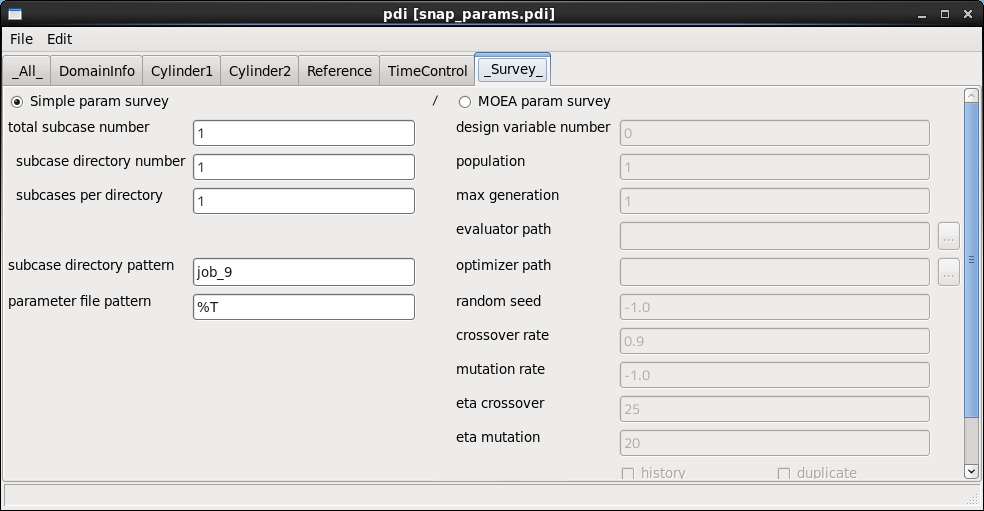
\includegraphics[width=360pt, bb=0 0 984 511]{figs/fig002.png}

図3 PDIのSurveyパネル
\end{center}

「Survey」タブ最上段のラジオボタンで「Simple param survey」が選択されている場合、「Survey」タブの左側が有効化されており、以下に示す項目を設定する事ができます。

全てのパラメータケース(サブケース)を組み合わせた数(全探査数)が「{\tt Total subcase number}」に表示されます。この数が0の場合は、パラメータ空間が縮退していることを意味し、ソルバ入力用のパラメータファイル生成を行うことはできません。

全探査数に対して、幾つの作業ディレクトリを作成するかを「{\tt subcase directory number}」に、または1つの作業ディレクトリにつき幾つのパラメータケースを割り当てるかを「{\tt subcases per directory}」に入力します。どちらか一方が入力されると、もう一方は自動的に更新されます。初期値は、1つの作業ディレクトリにつき1つのパラメータケース(作業ディレクトリ数=全探査数)です。(作業ディレクトリ数)×(作業ディレクトリ当りのパラメータケース数)≠(全探査数)の場合は、最後の作業ディレクトリに割り当てられるパラメータケース数で調整されます。

作業ディレクトリ名({\tt subcase directory pattern})、ソルバ入力用パラメータファイル名({\tt parameter file pattern})については、以下に示すキーワードを使用してパターンを設定します。

\begin{description}
\item[\%P] パラメータ組み合わせ
\item[\%Q] パラメータ組み合わせ(パラメータ名付き)
\item[\%T] テンプレートファイルのベース名\\
(テンプレートファイル名から末尾の\texttt{"}.template\texttt{"}, 
\texttt{"}.tmpl\texttt{"}, \texttt{"}.tmp\texttt{"}, \texttt{"}.tpl\texttt{"}を 除いたもの)
\item[\#D] 作業ディレクトリ通番
\item[\#J] サブケース通番
\item[\#T] ソルバ入力パラメータファイルが複数ある場合のファイル番号
\end{description}

\bigskip

尚、「Survey」タブ最上段のラジオボタンで「MOEA param survey」を選択すると、「Survey」タブの右側部分が有効になり、MOEA(多目的進化計算)による最適化の設定を行う事ができます。

PDIによるMOEA最適化については「3 MOEA最適化の設定」を参照して下さい。


\subsection{ソルバ入力用パラメータファイルの生成機能}

PDIによるソルバ入力用パラメータファイルの生成を行うには、パラメータ空間の設定とパラメータサーベイ方式の設定に加え、ソルバ入力パラメータテンプレートファイルの指定と、ソルバ種別の指定が必要です。

\subsubsection{ソルバ入力パラメータテンプレートファイルの指定}

ソルバ入力パラメータテンプレートファイルは、PDIの起動時に「{\tt -t}」オプションで指定することができます。「{\tt -t template\_file}」という形式で、複数指定することが可能です。

PDIをGUIモードで起動した場合、「Edit」メニューの「{\tt set parameter template file(s)}」から、ソルバ入力用パラメータテンプレートファイルの追加/削除を行うことができます。

このメニューを選択すると、下図に示すダイアログウインドウが表示されます。

\begin{center}
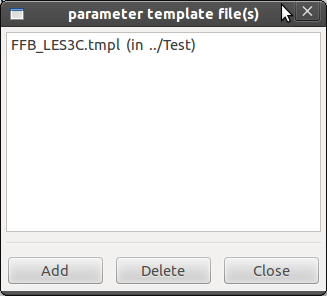
\includegraphics[width=184pt, bb=0 0 327 296]{figs/fig003.png}

図4 PDIのテンプレートファイル設定ダイアログ
\end{center}

このダイアログウインドウには、既に登録済みのソルバ入力用パラメータテンプレートファイルがリスト表示されています。このダイアログは「{Close」ボタンをクリックすると閉じられます。

「Add」ボタンをクリックすると、ファイル選択ダイアログが表示され、ここで選択したファイルがソルバ入力用パラメータテンプレートファイルととして追加されます。

リスト上で登録済みのソルバ入力用パラメータテンプレートファイルを選択状態にし、「Delete」ボタンをクリックすると、そのファイルの登録は解除されます。


\subsubsection{ソルバ種別の設定}

PDIでは、ソルバ入力用パラメータファイルの生成時に、パラメータスイープ実行のための設定ファイルを生成します。この設定ファイル中には、ソルバ実行の方法の記述も含まれるため、PDI上でソルバ種別の設定を行なっておく必要があります。

GUIモードで起動したPDIの「Edit」メニューから「{\tt select solver type}」を選択すると、下図に示すダイアログウインドウが表示されます。

\begin{center}
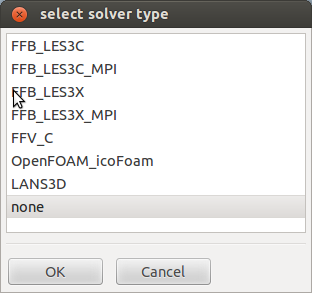
\includegraphics[width=176pt, bb=0 0 312 296]{figs/fig004.png}

図5 PDIのソルバ種別選択ダイアログ
\end{center}

ここには、PDIに予め登録されているソルバ種別の一覧がリスト表示され、リスト中の項目を選択状態にして「OK」ボタンをクリックすると、ソルバ種別の設定がおこなわれます。

現在、PDIに登録されているソルバ種別の設定を以下に示します。

\begin{tt}
\begin{tabular}{|l|l|l|}
\hline
ソルバ種別 & ソルバ実行コマンド & ソルバ入力パラメータファイル名パターン\tabularnewline
\hline
FFB\_LES3C & run\_les3c.sh & PARMLES3C\tabularnewline
\hline
FFB\_LES3C\_MPI & run\_les3c\_mpi.sh & PARMLES3C\tabularnewline
\hline
FFB\_LES3X & run\_les3x.sh & PARMLES3X\tabularnewline
\hline
FFB\_LES3X\_MPI & run\_les3x\_mpi.sh & PARMLES3X\tabularnewline
\hline
FFV & run\_ffv.sh \%T & \%T \tabularnewline
\hline
OpenFoam\_icoFoam & run\_openfoam.sh &  \tabularnewline
\hline
その他(none) & run.sh & 変更せず\tabularnewline
\hline
\end{tabular}
\end{tt}

上記の表中の「{\tt \%T}」は テンプレートファイルのベース名を表します。

また、パラメータスイープ実行のための設定ファイルにおいては、上記の表の「ソルバ実行コマンド」に示された実行ファイル(シェルスクリプト)がケースディレクトリ配下に存在することを前提としています。


\subsubsection{サブケースディレクトリとソルバ入力パラメータファイルの生成}

GUIモードで起動されたPDIでは、「File」メニューの「{\tt generate solver parameter file(s)}」を選択すると、パラメータスイープ用の作業ディレクトリ(サブケースディレクトリ)と、ソルバ入力用パラメータファイルの生成が行われます。

具体的には、以下に示す処理が行われます。\\

\textbf{(1) サブケースディレクトリの作成}

ケースディレクトリ配下に、作業ディレクトリ名パターンを展開したディレクトリが「{\tt subcase directory number}」個作成されます。作成しようとしているディレクトリが既に存在する場合は、そのディレクトリはそのまま流用されます。\\

\textbf{(2) ソルバ入力用パラメータファイルの作成}

作成したサブケースディレクトリの配下に、ソルバ入力用パラメータファイル名パターンを展開したファイル名で、ソルバ入力用パラメータファイルが作成されます。PDIは、指定されているソルバ入力パラメータテンプレートファイル中のマクロ記述をパラメータ値に置換することで、ソルバ入力用パラメータファイルを生成します。複数のンプレートファイルが指定されている場合、それらすべてに対応するソルバ入力用パラメータファイルが作成されます。

作成しようとしているソルバ入力用パラメータファイルが既に存在する場合は、そのファイルは上書きされます。\\

\textbf{(3) ワークフロー実行用パラメータ設定ファイルの作成}

実際のソルバ実行を含むパラメータスイープ/パラメータサーベイの実行は、ケースワークフローからLuaスクリプトとして実行されます。

PDIは、ソルバ入力用パラメータファイルの生成時に、Luaスクリプトファイルとして、ケースディレクトリ配下に{\tt pdi\_generated.lua}というファイルを作成します。同名のファイルが既に存在する場合、そのファイルは上書きされます。

{\tt pdi\_generated.lua}は、ケースワークフローファイル({\tt cwf.lua})から{\tt require}され、関数{\tt EXEC\_PARAMSWEEP(...)}が呼び出されることを前提として記述されています。\\

\textbf{(4) パラメータリストファイルの作成}

パラメータリストファイルは、現在のパラメータ空間設定の下で実行されるパラメータスイープのパラメータ値を記述したCSV形式のテキストファイルです。

PDIは、ソルバ入力用パラメータファイルの生成時に、パラメータリストファイルをケースディレクトリ配下に {\tt param\_list.csv}というファイル名で作成します。同名のファイルが既に存在する場合、そのファイルは上書きされます。\\


\subsection{パラメータ空間設定情報の保存}

PDIは終了時に、その時点でのパラメータ空間設定情報とパラメータサーベイ方式設定情報を、ケースディレクトリ配下に {\tt snap\_params.pdi}というファイル名で保存します。既にこのファイルが存在する場合、ファイルは上書きされます。

{\tt snap\_params.pdi}ファイルが存在するディレクトリがケースディレクトリとして指定({\tt -x})された場合、パラメータ記述ファイルの指定({\tt -d})がなくてもPDIはパラメータ空間設計を行うことが可能です(この場合、ログにはワーニングが出力されます)。また、パラメータ記述ファイルの指定が行われた場合は、パラメータ記述ファイルのロード後に {\tt snap\_params.pdi}ファイルに保存された情報の反映を行います。

ただし、指定されたパラメータ記述ファイルと、{\tt snap\_params.pdi}ファイルに保存されているパラメータ記述ファイル名が異なる場合は、{\tt snap\_params.pdi}ファイルの内容は無視されます。


\subsection{バッチモードでのPDI実行}

PDI起動時に「{\tt -b}」または「{\tt -B}」オプションを指定すると、PDIはGUIウインドウを表示せず、バッチモードで実行されます。

バッチモードでのPDI実行は主に、以前に設定されたパラメータスイープにおけるパラメータ空間の変更を行うために行います。PDI起動時に「{\tt -p}」オプションで1個ないし複数個のパラメータ値を変更することにより、{\tt ケースディレクトリ/snap\_params.pdi}ファイルに保存された前回設定のパラメータ空間が更新されます。ただしこの場合は、前回パラメータ空間を設定した際と同じケースディレクトリが指定されていることが必要です。

\begin{description}
\item[実行の例] {\ }\\
{\tt pdi  -x case01  -p Re:100/200/10}\\
{\tt (ケースディレクトリ「case01」において、「Re」という名前のパラメータを、100から200まで10刻みでスイープさせる)}
\end{description}

PDIの「{\tt -p}」オプション指定方法の詳細は、2.1章を参照してください。

\newpage
\section{MOEA最適化の設定}

\subsection{概要}

工学的な最適化問題は、最適化の対象である目的関数が複数(一般的には2個以上)存在する多目的最適化問題である場合が多く、しかもそれらは相反する性質を持つ場合も珍しくありません。

JAXA(宇宙航空研究開発機構\footnote{\tt http://www.jaxa.jp})が開発したCheetahは、生物の進化のメカニズムを模倣した進化的アルゴリズム(EA)を多目的最適化問題に適用するMOEA(多目的進化計算)のソフトウエアフレームワークです。

PDIでは、設定したパラメータ空間内での最適化計算をCheetahを使用して実行するためのスクリプトの生成と、実行環境を設定する機能を含んでいます。

本章では、PDIによるMOEAのパラメータ設定と実行方法について説明します。

尚、JAXAによる多目的設計探査に関する詳細については、以下のURLを参照して下さい。
\begin{quote}
{\tt http://flab.eng.isas.jaxa.jp/monozukuri/mode/index.html}
\end{quote}


\subsection{MOEAの設定方法}

MOEAの設定は「Survey」タブを選択し、最上段の「MOEA param survey」ラジオボタンを選択する事で行えるようになります。選択すると「Survey」タブ上で有効化されている部分が変更され、MOEAの設定が可能になります。

\begin{center}
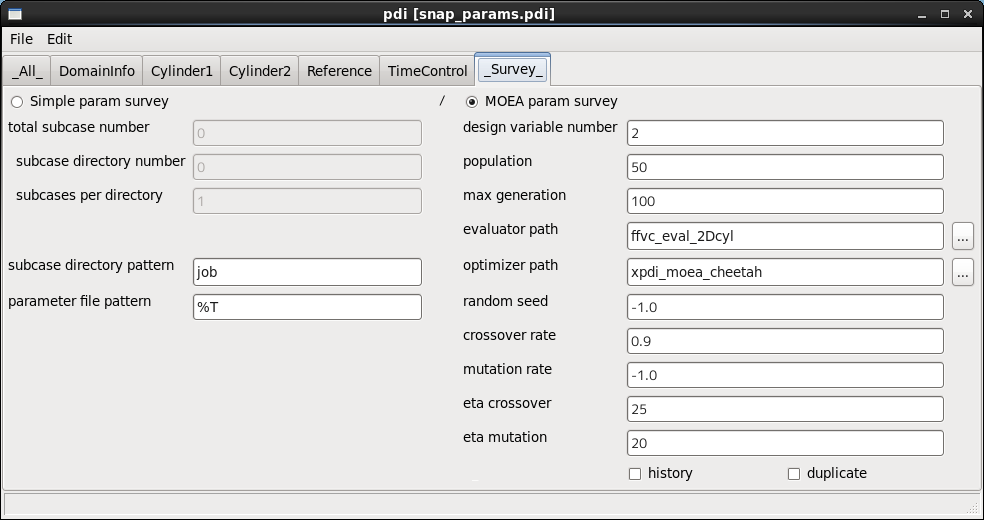
\includegraphics[width=360pt, bb=0 0 984 520]{figs/fig005.png}

図6 PDIのSurveyパネル(「MOEA param survey」選択時)
\end{center}

ここでは、以下に示す項目を設定します。

\begin{description}
\item[subcase directory pattern] {\ }\\
作業ディレクトリ名のパターン(ベース部分)を指定します。
「Simple param survey」選択時と指定方法は同じですが、パターン表現用のキーワード(\%P, \%Q, \#D 等)は全て空文字列と置き換えられ(取り除かれ)、残った文字列を作業ディレクトリ名のベース部分として使用します。

実際の作業ディレクトリは、ケースディレクトリ配下に「ベース部分\_整数」という形式で、population(後述)個作成されます。\\

\item[parameter file pattern] {\ }\\
各作業ディレクトリ配下に作成される、ソルバ入力用パラメータファイルのファイル名パターンを指定します。「Simple param survey」選択時と指定方法は同じです。\\

\item[design variable number] {\ }\\
MOEAにおける設計変数となるパラメータ項目の数が表示されます。この値は変更できません。

PDIにおけるMOEA param sweepでは、「レンジ指定」を選択し、範囲(最小/最大値)を設定したint型またはreal型のパラメータを設計変数として扱います。「design variable number」欄には、この条件を満たすパラメータ項目の数が表示されます。

この欄の値が0の場合は、探索すべき設計変数が存在しない事を意味し、MOEA計算は行えません。

尚、「Survey」タブで「MOEA param sweep」を選択した場合、各パラメータ項目設定タブ上では「レンジ指定」を表す「sweep range」の表記が「search range」に変わり、パラメータの刻み幅入力欄(delta)は有効精度の入力欄(precision)に変わります(下図参照)。

\begin{center}
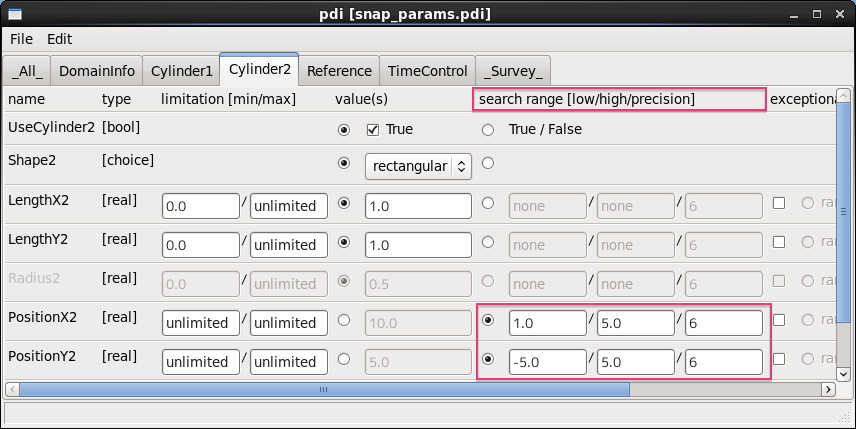
\includegraphics[width=320pt, bb=0 0 856 429]{figs/fig006.png}

図7 PDIのパラメータ設定パネル(「MOEA param survey」選択時)
\end{center}

\item[population] {\ }\\
MOEA計算における個体数を設定します。ここで設定した個数だけ作業ディレクトリが作成されます。4の倍数である必要があります。また、0以下の値は設定できません。

\item[max generation] {\ }\\
MOEA計算における世代数を設定します。ここで設定した回数だけ\par
\begin{center}
\{ソルバー実行 \ ⇒ \ パラメータ値(設計変数)の進化計算\}
\end{center}\par
がループ実行されます。0以下の値は設定できません。

\item[evaluator path] {\ }\\
MOEA計算における評価モジュール(evaluator)のパスを設定します。
入力欄の右の「...」ボタンをクリックするとファイル選択ダイアログが表示され、ここでファイルを選択すると入力欄に反映されます。

評価モジュールは、ソルバーの実行結果から目的関数の値を計算する外部プログラムであり、最適化問題毎に使用者が用意する必要があります。評価モジュールの仕様(インターフェースの詳細)については、「5 外部プログラムの形式」を参照して下さい。

\item[optimizer path] {\ }\\
MOEA計算における進化計算モジュール(optimizer)のパスを設定します。
入力欄の右の「...」ボタンをクリックするとファイル選択ダイアログが表示され、ここでファイルを選択すると入力欄に反映されます。

進化計算モジュールは、目的関数の値から、次の世代の設計変数を生成する外部プログラムであり、PDIではCheetahを使用した進化計算モジュール({\tt xpdi\_moea\_cheetah})を提供しています。進化計算モジュールの仕様(インターフェースの詳細)については、「5 外部プログラムの形式」を参照して下さい。

\item[random seed] {\ }\\
MOEA計算において使用する乱数の種を設定します。有効な値は0.0〜1.0ですが、負値を設定した場合は乱数を用いて設定されます。

\item[crossover rate] {\ }\\
MOEA計算における交叉率を設定します。有効な値は0.0〜1.0です。

\item[mutation rate] {\ }\\
MOEA計算における突然変異率を設定します。有効な値は0.0〜1.0ですが、負値を設定した場合は自動的に$(1.0 / 設計変数個数)$に設定されます。

\item[eta crossover] {\ }\\
MOEA計算における交叉のdistribution indexを設定します。有効な値は5〜40です。

\item[eta mutation] {\ }\\
MOEA計算における突然変異のdistribution indexを設定します。有効な値は5〜50です。

\item[history] {\ }\\
MOEA計算において、全評価個体の履歴ファイル(interface/history.txt)を作成するかどうかを設定します。

\item[duplicate] {\ }\\
MOEA計算において、重複する設計点を作成するかどうかを設定します。



\end{description}


\subsection{MOEA実行環境の生成}

前節に示したMOEAの設定を行い、「File」メニューの「{\tt generate solver parameter file(s)}」を選択すると、MOEA計算実行用の環境が生成されます。

ケースディレクトリ配下に以下のようなディレクトリ・ファイルが生成されます。

\begin{verbatim}
[ケースディレクトリ]
  ├── (cwf.lua)           (ケースワークフローファイル)
  ├── (input_data)
  │     └── (run.sh)     (ソルバー実行スクリプト)
  ├── cfg
  │     ├── moea.cfg     (Cheetah用コンフィグレーションファイル)
  │     └── mop.cfg      (目的関数定義ファイル)
  ├── job_{0 〜 個体数-1} (サブケースディレクトリ)
  │     └── run.sh       (ソルバー実行スクリプト)
  ├── interface           (Cheetah作業用ディレクトリ)
  ├── moea_out            (Cheetah出力用ディレクトリ)
  └── pdi_generated.lua   (ワークフロー記述Luaファイル)
\end{verbatim}

ソルバー実行スクリプトは、{\tt input\_data}ディレクトリ配下から、全てのサブケースディレクトリ配下にコピーされます。ファイル名はソルバー種別によって異なります。

ワークフロー記述Luaファイル({\tt pdi\_generated.lua})は、ケースワークフローファイル({\tt cwf.lua})から{\tt require}され、関数{\tt EXEC\_PARAMSWEEP(...)}が呼び出されることを前提として記述されています。

尚、ケースワークフローファイルおよび{\tt input\_data}ディレクトリは、ケースディレクトリに事前に用意されている事が前提です。


\subsection{MOEAの実行}

PDIで生成したMOEA実行環境は、ケースディレクトリでケースワークフローを実行する事で実行されます。この実行には、Xjob(hpcpfGUIに付属)のライブラリパスが環境変数{\tt LUA\_PATH}に設定されている事が必要です\footnote{hpcpfGUIから実行される場合は、ディレクトリ移動と環境変数設定は自動で行われています。}。

\begin{verbatim}
  $ cd "ケースディレクトリ"
  $ export LUA_PATH="hpcpfGUIインストールディレクトリ"/lib
  $ lua cwf.lua
\end{verbatim}

以下に、ケースワークフローが実行された際に行われるMOEA計算処理の概要を示します。

\begin{enumerate}
\item optimizer({\tt xpdi\_moea\_cheetah})を世代番号0で実行します。
これにより、探査空間内のランダムな設計点が個体数個生成され、{\tt interface/pop\_vars\_eval.txt}ファイルに出力されます。

\item 内部コマンド{\tt xpdi\_genparam}を実行します。
これにより、内部的にPDIがバッチモードで実行され、各サブケースディレクトリ配下にそるバー入力パラメータファイルが生成されます。

\item 個体数個分のソルバー実行ジョブが発行されます。

\item 全てのジョブの完了後、evaluatorが実行されます。
これにより、各ジョブ毎の目的関数(および制約条件)が計算され、{\tt interface/pop\_objs\_eval.txt}ファイル(および{\tt pop\_cons\_eval.txt})に出力されます。

\item 世代番号を$+1$し、最大世代数回、処理1から繰り返します。
\end{enumerate}

計算結果は、{\tt moea\_out/allpop.txt}に出力されます。


\newpage
\section{ファイルフォーマット}

\subsection{パラメータ定義ファイル}

パラメータ定義ファイルは、XML形式のテキストファイルとして記述されます。

以下に、構成要素となるXMLノードの記述方式を示します。\\

\textbf{(1) トップレベルノード}

パラメータ定義ファイルのトップレベルノードは\texttt{<hpcpf\_paramdesc>}です。

このノード配下に記述された内容だけがPDIの処理対象となります。

\vspace{8pt}
\leftskip=12pt
\textbf{[記述形式]}

\leftskip=42pt
\texttt{<hpcpf\_paramdesc  [classification="snapshot"]>} 
   
...

\texttt{</hpcpf\_paramdesc>}

\vspace{8pt}
\leftskip=0pt
\texttt{<hpcpf\_paramdesc>}ノードには、{\tt classification}属性としてキーワード\texttt{"snapshot"}を記述することができます。このキーワードが記述されたパラメータ定義ファイルは、パラメータ空間設定情報を保存したスナップショットデータファイルと認識されます。スナップショットデータファイルは通常、PDIの終了時にケースディレクトリ配下に{\tt snap\_params.pdi}というファイル名で作成されます。

\vspace{12pt}
\textbf{(2) パラメータ記述ノード}

パラメータ項目の記述には、\texttt{<param>}ノードを使用します。

\vspace{8pt}
\leftskip=12pt
\textbf{[記述形式]}

\leftskip=42pt
\texttt{<param name="パラメータ名"  type="パラメータタイプ" 
 [disable="True\textbar{}False"]>}    

\parindent=14pt
\{パラメータ説明文\}

\{サブノード群\}

\parindent=0pt
\texttt{</param>}

\vspace{8pt}
\leftskip=0pt
\texttt{<param>}ノードには、name属性およびtype属性を記述する必要があります。

name属性には、パラメータ名を記述します。

type属性には、以下のいずれかのパラメータタイプを記述します。

\parindent=18pt
int 整数

real 実数

bool 真偽値(True \textbar{} False)

string 文字列

choice 文字列候補

\parindent=0pt
\texttt{<param>}ノードには、{\tt disable}属性を記述することができます。{\tt disable}属性には\texttt{"True"}または\texttt{"False"}のキーワードを記述し、{\tt True}の場合はそのパラメータは無効化されます。記述を省略した場合、{\tt disable}属性は\texttt{"False"}とみなされます。

\vspace{12pt}
\texttt{<param>}ノード配下には、パラメータ説明のテキストと、複数のサブノードを記述することができます。

\texttt{<param>}ノード配下の最初のテキストは、パラメータ説明の記述として扱われます。

\texttt{<param>}ノード配下に記述できるサブノードについては、以下の説明を参照して下さい。

\vspace{12pt}
\textbf{(3) パラメータ記述サブノード}

以下は、\texttt{<param>}ノード配下に記述できるサブノードの説明です。

\vspace{12pt}
\textbf{(3-a) \texttt{<item>}ノード }

\parindent=3pt
\texttt{<item>}ノードは、\texttt{<param>}ノードの{\tt type}属性が\texttt{"choice"}の場合の、文字列候補の1つを記述するノードで、\texttt{<param>}ノード配下に複数(選択候補数)個記述できます。

\vspace{8pt}
\parindent=0pt
\leftskip=12pt
\textbf{[記述形式]}

\leftskip=42pt
\texttt{<item>文字列候補1</item>}

\texttt{<item>文字列候補2</item>}

\vspace{8pt}
\leftskip=0pt
\texttt{<param>}ノードの{\tt type}属性が\texttt{"choice"}意外の場合は、\texttt{<item>}ノードの記述は無視されます。

\vspace{12pt}
\textbf{(3-b) \texttt{<range>}ノード・\texttt{<minmax>}ノード}

\texttt{<range>}ノードおよび\texttt{<minmax>}ノードは、\texttt{<param>}ノードのtype属性が\texttt{"int"}または\texttt{"real"}の場合の、値域を記述するノードです。

\vspace{8pt}
\leftskip=12pt
\textbf{[記述形式]}

\leftskip=42pt
\texttt{<range  min="最小値"  max="最大値" />}

\texttt{<minmax  min="最小値"  max="最大値" />}

\vspace{8pt}
\leftskip=0pt
{\tt min}属性に値域の最小値を、{\tt max}属性に最大値を記述します。{\tt min}属性または{\tt max}属性の記述を省略した場合、省略された方向の値制限は無しになります。また、\texttt{<range>}ノードおよび\texttt{<minmax>}ノードの記述自体を省略すると、値域制限は無しになります。

\vspace{12pt}
\textbf{(3-c) \texttt{<value>}ノード}

\texttt{<}value\texttt{>}ノードは、パラメータ値の初期値を記述するノードです。

\vspace{8pt}
\leftskip=12pt
\textbf{[記述形式]}

\leftskip=42pt
\texttt{<value>}パラメータ値\texttt{</value>}

\vspace{8pt}
\leftskip=0pt
\texttt{<value>}ノードの記述を省略した場合、パラメータ値の初期値は\texttt{<param>}ノードの{\tt type}属性に応じ、以下に示すようになります。

\parindent=18pt
int \texttt{"}0\texttt{"}

real \texttt{"}0.0\texttt{"}

bool \texttt{"}False\texttt{"}

string \texttt{"}\texttt{"} (空文字列)

choice \texttt{"}0\texttt{"}(先頭の候補)

\parindent=0pt
\texttt{<param>}ノードの{\tt type}属性が\texttt{"}int\texttt{"}または\texttt{"}real\texttt{"}の場合は、パラメータ値は空白で区切って複数の値を列挙することができます。

\vspace{12pt}
\textbf{(3-d) \texttt{<useRange>}ノード}

\texttt{<useRange>}ノードは、\texttt{<param>}ノードのパラメータ値を値域・刻み幅指定で定義するかどうかを記述するノードです。

\vspace{8pt}
\leftskip=12pt
\textbf{[記述形式]}

\leftskip=42pt
\texttt{<useRange> True \textbar{} False </useRange>}

\vspace{8pt}
\leftskip=0pt
\texttt{"False"}の場合、\texttt{<value>}ノード記述に従ってパラメータ値を設定します。

\texttt{"True"}の場合、\texttt{<value>}ノードの記述は参照せず、次項で説明する\texttt{<sweepRange>}ノードの記述に従ってパラメータ値を設定します。ただし、\texttt{<param>}ノードのtype属性が\texttt{"bool"}の場合はパラメータ値が\texttt{"True"}と\texttt{"False"}の2サブケースとして、\texttt{<param>}ノードの{\tt type}属性が\texttt{"choice"}の場合は 
\texttt{<item>}ノードで記述した全ての候補をパラメータ値とするサブケースが設定されます。\texttt{<param>}ノードの{\tt type}属性が\texttt{"string"}の場合、\texttt{<useRange>}ノードの値は無視され、常に\texttt{<value>}ノードの記述に従ってパラメータ値が設定されます。

\texttt{<useRange>}ノードの記述を省略した場合のデフォルト値は\texttt{"False"}です。

\vspace{12pt}
\textbf{(3-e) \texttt{<sweepRange>}ノード}

\texttt{<sweepRange>}ノードは、\texttt{<useRange>}ノードの値が\texttt{"True"}の場合の、値域・刻み幅指定によるパラメータ値の設定を記述するノードです。

\vspace{8pt}
\leftskip=12pt
\textbf{[記述形式]}

\leftskip=42pt
\texttt{<sweepRange  min="最小値"  max="最大値"  delta="刻み幅" />}

\vspace{8pt}
\leftskip=0pt
{\tt min}属性に値域の最小値を、{\tt max}属性に最大値を、{\tt delta}属性に刻み幅を記述します。これらの属性の記述は省略できません。

尚、\texttt{<sweepRange>}ノードの記述は\texttt{<param>}ノードの{\tt type}属性が\texttt{"int"}または\texttt{"real"}の場合以外は無視されます。

\vspace{12pt}
\textbf{(3-f) \texttt{<useExcept>}ノード}

\texttt{<useExcept>}ノードは、\texttt{<param>}ノードのパラメータ値に対する除外値指定を参照するかどうかを記述するノードです。

\vspace{8pt}
\leftskip=12pt
\textbf{[記述形式]}

\leftskip=42pt
\texttt{<useExcept> True \textbar{} False </useExcept>}

\vspace{8pt}
\leftskip=0pt
\texttt{"False"}の場合、除外値の指定は参照されません。

\texttt{"True"}の場合、次項以降で説明する\texttt{<except>}ノードまたは\texttt{<exceptRange>}ノードの記述に従って除外値を設定します(最後に記述された\texttt{<except>}ノードまたは\texttt{<exceptRange>}ノードが有効になります)。

\vspace{12pt}
\textbf{(3-g) \texttt{<except>}ノード}

\texttt{<except>}ノードは、\texttt{<param>}ノードのパラメータ値に対する除外値を直接記述するノードです。

\vspace{8pt}
\leftskip=12pt
\textbf{[記述形式]}

\leftskip=42pt
\texttt{<except>}除外値\texttt{</except>}

\vspace{8pt}
\leftskip=0pt
除外値は、空白で区切って複数指定することが可能です。
尚、\texttt{<except>}ノードの記述は\texttt{<param>}ノードの{\tt type}属性が\texttt{"int"}または\texttt{"real"}の場合以外は無視されます。

\vspace{12pt}
\textbf{(3-h) \texttt{<exceptRange>}ノード}

\texttt{<exceptRange>}ノードは、\texttt{<param>}ノードのパラメータ値に対する除外値を範囲で指定するノードです。

\vspace{8pt}
\leftskip=12pt
\textbf{[記述形式]}

\leftskip=42pt
\texttt{<except  min="最小値"  max="最大値" />}

\vspace{8pt}
\leftskip=0pt
{\tt min}属性に除外範囲の最小値を、{\tt max}属性に最大値を記述します。{\tt min}属性または{\tt max}属性の記述を省略した場合、省略された方向の除外範囲制限は無しになります。

尚、\texttt{<exceptRange>}ノードの記述は\texttt{<param>}ノードの{\tt type}属性が\texttt{"int"}または\texttt{"real"}の場合以外は無視されます。

\vspace{12pt}
\textbf{(3-i) \texttt{<arithPrec>}ノード}

\texttt{<arithPrec>}ノードは、\texttt{<param>}ノードのパラメータをMOEAの設計変数として使用する場合に、変数の精度(小数点以下の桁数)を指定するノードです。

\vspace{8pt}
\leftskip=12pt
\textbf{[記述形式]}

\leftskip=42pt
\texttt{<arithPrec>桁数</arithPrec>}

\vspace{8pt}
\leftskip=0pt
記述を省略した場合、変数の精度は\texttt{<param>}ノードの{\tt type}属性が\texttt{"int"}の場合は0、\texttt{"real"}の場合は6になります。

尚、\texttt{<arithPrec>}ノードの記述は\texttt{<param>}ノードの{\tt type}属性が\texttt{"int"}または\texttt{"real"}の場合以外は無視されます。

\vspace{12pt}
\textbf{(3-j) 依存関係記述ノード}

\texttt{<param>}ノード配下には、他のパラメータ項目との依存関係を示すためのサブノードを記述することができます。依存関係記述ノードの記述方法については、(5)を参照して下さい。

\vspace{12pt}
\textbf{(4) パラメータのグルーピング}

複数のパラメータ項目をグループとしてまとめるため、\texttt{<group>}ノードを記述することができます。

\vspace{8pt}
\leftskip=12pt
\textbf{[記述形式]}

\leftskip=42pt
\texttt{<group name="グループ名">}    

\parindent=14pt
\{パラメータノード群\}

\parindent=0pt
\texttt{</group>}

\vspace{8pt}
\leftskip=0pt
\texttt{<group>}ノードには、{\tt name}属性を記述する必要があります。{\tt name}属性には、グループ名を記述します。

\vspace{12pt}
\texttt{<group>}ノード配下には、グルーピングするパラメータ項目の\texttt{<param>}ノードを複数記述することができます。グルーピングされたパラメータ群は、PDIサブシステム上でパラメータ値の設定を行う際に、まとめて参照出来るように処理されます。

\vspace{12pt}
\textbf{(5) 依存関係の記述}

\vspace{12pt}
\textbf{(5-a) \texttt{<depend>}ノード}

\texttt{<depend>}ノードは、このノードを配下に持つ\texttt{<param>}ノード(親ノード)の記述が、他の\texttt{<param>}ノードのパラメータ値に依存することを示すためのノードです。

\vspace{8pt}
\leftskip=12pt
\textbf{[記述形式]}

\leftskip=42pt
\texttt{<depend target="パラメータ項目名" [target2="パラメータ項目名2"]>} 
   

\parindent=14pt
\texttt{<cond>}ノード

\parindent=0pt
\texttt{</depend>}

\vspace{8pt}
\leftskip=0pt
\texttt{<depend>}ノードには、依存する\texttt{<param>}ノードの名前({\tt name}属性)を\texttt{target}および\texttt{target2}属性に記述する必要があります。ここに記述した\texttt{<param>}ノードが存在しない場合、この\texttt{<depend>}ノードの記述は無視されます。\texttt{target}属性は必ず記述する必要がありますが、\texttt{target2}属性の記述は無くても構いません。

\texttt{<depend>}ノード配下には、依存する\texttt{<param>}ノードとの関係条件を記述する\texttt{<cond>}ノードをサブノードとして記述します。

\vspace{12pt}
尚、\texttt{<depend>}ノードは\texttt{<param>}ノードの配下にのみサブノードとして記述することができます。

\vspace{12pt}
\textbf{(5-b) \texttt{<cond>}ノード}

\texttt{<cond>}ノードは、パラメータ項目間の依存関係の条件を記述するためのノードで、\texttt{<depend>}ノードのサブノードとして記述します。

\vspace{8pt}
\leftskip=12pt
\textbf{[記述形式]}

\leftskip=42pt
\texttt{<cond>}「条件式」 ? 「真文」 : 「偽文」\texttt{</cond>}

\vspace{8pt}
\leftskip=0pt
ここで、「条件式」は以下の形式で記述します。
\begin{quote}
「ターゲット」「演算子」「値」\\
「ターゲット」「演算子」「値」「結合演算子」「ターゲット2」「演算子2」「値2」
\end{quote}

「ターゲット」には固定文字列として\texttt{"VAL"}を記述します。

\vspace{12pt}

「演算子」には、以下のいずれかを記述します。

\leftskip=10pt
{\tt 「==」または「EQ」}

{\tt 「!=」または「NE」}

「\texttt{<}」または「{\tt LT}」

「\texttt{<=}」または「{\tt LE}」

「\texttt{>}」または「{\tt GT}」

「\texttt{>=}」または「{\tt GE}」

\leftskip=0pt
(一部のPython/XML処理系では、XMLタグ以外で「\texttt{<}」文字を使用出来ません。)

\medskip
\texttt{<cond>}ノードの上位の\texttt{<depend>}ノードで\texttt{target2}属性が指定されている場合、ここで指定された\texttt{<param>}ノードの値を「値2」として、2つの条件式を「結合演算子」で結合する事が出来ます。

「結合演算子」以下のいずれかを記述します。

\leftskip=10pt
{\tt 「\&\&」または「AND」}

{\tt 「||」または「OR」}


\vspace{12pt}

ターゲットに指定されたのパラメータのtype属性が\texttt{"string"}または\texttt{"choice"}の場合、記述できる演算子は「\texttt{==}」、「\texttt{!=}」、「\texttt{<}」および「\texttt{>}」のみで、「\texttt{==}」が文字列の一致を、それ以外は文字列の不一致を表します。

「真文」および「偽文」には、以下のいずれかを記述することができます。

\leftskip=10pt
\begin{tt}
「enable」

「disable」

「set value=\texttt{"}値\texttt{"}」

「set range=\texttt{"}最小値  最大値\texttt{"}」

「set sweep=\texttt{"}最小値  最大値  刻み幅\texttt{"}」
\end{tt}
\leftskip=0pt
ここで、「{\tt enable}」および「{\tt disable}」は、このパラメータ項目の有効化/無効化を表します。また、「{\tt set value}」、「{\tt set range}」および「{\tt set sweep}」は、このパラメータ項目の値、値域およびパラメータスイープ範囲と刻み幅を設定(変更)することを意味します。

\vspace{12pt}
\textbf{(6) パラメータサーベイ方式設定情報}

パラメータサーベイ方式の設定情報は、\texttt{<survey>}ノードに記述されます。

\vspace{8pt}
\leftskip=12pt
\textbf{[記述形式]}

\leftskip=42pt
\texttt{<survey>}    

\parindent=14pt
\{サブノード群\}

\parindent=0pt
\texttt{</survey>}

\vspace{8pt}
\leftskip=0pt
\texttt{<survey>}ノード配下に記述できるサブノードについては、以下の説明を参照して下さい。

\vspace{12pt}
\textbf{(6-a) \texttt{<wdPattern>}ノード}

\texttt{<wdPattern>}ノードは、サブケースジョブの作業ディレクトリ名のパターンを記述するノードです。

\vspace{8pt}
\leftskip=12pt
\textbf{[記述形式]}

\leftskip=42pt
\texttt{<wdPattern>}作業ディレクトリ名パターン\texttt{</wdPattern>}

\vspace{12pt}
\leftskip=0pt
\textbf{(6-b) \texttt{<pfPattern>}ノード}

\texttt{<pfPattern>}ノードは、サブケースジョブのソルバ入力パラメータファイル名のパターンを記述するノードです。

\vspace{8pt}
\leftskip=12pt
\textbf{[記述形式]}

\leftskip=42pt
\texttt{<pfPattern>}ソルバ入力パラメータファイル名パターン\texttt{</pfPattern>}

\vspace{12pt}
\leftskip=0pt
\textbf{(6-c) \texttt{<moeaMode>}ノード}

\texttt{<moeaMode>}ノードは、MOEA計算を有効にするかどうかを記述するノードです。

\vspace{8pt}
\leftskip=12pt
\textbf{[記述形式]}

\leftskip=42pt
\texttt{<moeaMode> True \textbar{} False </moeaMode>}

\vspace{8pt}
\leftskip=0pt
\texttt{"True"}が記述された場合、MOEA計算を有効に設定します。

\vspace{12pt}
\leftskip=0pt
\textbf{(6-d) \texttt{<moea>}ノード}

\texttt{<moea>}ノードは、MOEA計算を実行する際の各種設定値を記述するノードです。

\vspace{8pt}
\leftskip=12pt
\textbf{[記述形式]}

\leftskip=42pt
\texttt{<moea>}

\parindent=14pt
\{サブノード群\}

\parindent=0pt
\texttt{</moea>}

\vspace{8pt}
\leftskip=0pt
\texttt{"<moea>"}ノード配下には、MOEA計算用の各種設定を記述するための各種ノード群をサブノードとして記述します。

\vspace{12pt}
\textbf{(6-e) \texttt{<population>}ノード}

\texttt{<population>}ノードは、MOEA計算の個体数を記述するノードです。

\vspace{8pt}
\leftskip=12pt
\textbf{[記述形式]}

\leftskip=42pt
\texttt{<population>}個体数\texttt{</population>}

\vspace{8pt}
\leftskip=0pt
個体数は1以上の4の倍数の整数で指定します。MOEA計算を行う場合、このノードの記述は省略できません。

\vspace{12pt}
\textbf{(6-f) \texttt{<maxGeneration>}ノード}

\texttt{<maxGeneration>}ノードは、MOEA計算の最大世代数を記述するノードです。

\vspace{8pt}
\leftskip=12pt
\textbf{[記述形式]}

\leftskip=42pt
\texttt{<maxGeneration>}最大世代数\texttt{</maxGeneration>}

\vspace{8pt}
\leftskip=0pt
最大世代数は1以上の整数で指定します。

\texttt{<maxGeneration>}ノードの記述を省略した場合のデフォルト値は1です。


\vspace{12pt}
\textbf{(6-g) \texttt{<evaluator>}ノード}

\texttt{<evaluator>}ノードは、MOEA計算における評価モジュール(evaluatorプログラム)の実行パスを記述するノードです。

\vspace{8pt}
\leftskip=12pt
\textbf{[記述形式]}

\leftskip=42pt
\texttt{<evaluator>}evaluatorプログラムの実行パス\texttt{</evaluator>}

\vspace{8pt}
\leftskip=0pt
evaluatorプログラムの実行パスは、絶対パスか、ケースディレクトリからの相対パスで指定します。

\vspace{12pt}
\textbf{(6-h) \texttt{<optimizer>}ノード}

\texttt{<optimizer>}ノードは、MOEA計算における最適化モジュール(optimizerプログラム)の実行パスを記述するノードです。

\vspace{8pt}
\leftskip=12pt
\textbf{[記述形式]}

\leftskip=42pt
\texttt{<optimizer>}optimizerプログラムの実行パス\texttt{</optimizer>}

\vspace{8pt}
\leftskip=0pt
optimizerプログラムの実行パスは、絶対パスか、ケースディレクトリからの相対パスで指定します。

\texttt{<optimizer>}ノードの記述を省略した場合のデフォルト値は、PDI付属のCheetahを使用するプログラム({\tt xpdi\_moea\_cheetah})です。

\vspace{12pt}
\textbf{(6-i) \texttt{<randSeed>}ノード}

\texttt{<randSeed>}ノードは、MOEA計算における乱数の種を記述するノードです。

\vspace{8pt}
\leftskip=12pt
\textbf{[記述形式]}

\leftskip=42pt
\texttt{<randSeed>}乱数の種\texttt{</randSeed>}

\vspace{8pt}
\leftskip=0pt
乱数の種は0.0 〜 1.0の実数で指定します。
負値が指定された場合は自動で指定されます。

\texttt{<randSeed>}ノードの記述を省略した場合のデフォルト値は-1.0です。

\vspace{12pt}
\textbf{(6-j) \texttt{<crossoverRate>}ノード}

\texttt{<crossoverRate>}ノードは、MOEA計算における交叉率を記述するノードです。

\vspace{8pt}
\leftskip=12pt
\textbf{[記述形式]}

\leftskip=42pt
\texttt{<crossoverRate>}交叉率\texttt{</crossoverRate>}

\vspace{8pt}
\leftskip=0pt
交叉率は0.0 〜 1.0の実数で指定します。

\texttt{<crossoverRate>}ノードの記述を省略した場合のデフォルト値は0.9です。

\vspace{12pt}
\textbf{(6-k) \texttt{<mutationRate>}ノード}

\texttt{<mutationRate>}ノードは、MOEA計算における突然変異率を記述するノードです。

\vspace{8pt}
\leftskip=12pt
\textbf{[記述形式]}

\leftskip=42pt
\texttt{<mutationRate>}突然変異率\texttt{</mutationRate>}

\vspace{8pt}
\leftskip=0pt
突然変異率は0.0 〜 1.0の実数で指定します。

\texttt{<mutationRate>}ノードの記述を省略した場合のデフォルト値は$(1.0 / 設計変数個数)$です。

\vspace{12pt}
\textbf{(6-l) \texttt{<etaCrossover>}ノード}

\texttt{<etaCrossover>}ノードは、MOEA計算における交叉のdistribution indexを記述するノードです。

\vspace{8pt}
\leftskip=12pt
\textbf{[記述形式]}

\leftskip=42pt
\texttt{<etaCrossover>}distribution index\texttt{</etaCrossover>}

\vspace{8pt}
\leftskip=0pt
distribution indexは5 〜 40の整数で指定します。

\texttt{<etaCrossover>}ノードの記述を省略した場合のデフォルト値は25です。

\vspace{12pt}
\textbf{(6-m) \texttt{<etaMutation>}ノード}

\texttt{<etaMutation>}ノードは、MOEA計算における突然変異のdistribution indexを記述するノードです。

\vspace{8pt}
\leftskip=12pt
\textbf{[記述形式]}

\leftskip=42pt
\texttt{<etaMutation>}distribution index\texttt{</etaMutation>}

\vspace{8pt}
\leftskip=0pt
distribution indexは5 〜 50の整数で指定します。

\texttt{<etaMutation>}ノードの記述を省略した場合のデフォルト値は20です。

\vspace{12pt}
\textbf{(6-n) \texttt{<history>}ノード}

\texttt{<history>}ノードは、MOEA計算において全評価個体の履歴ファイル({\tt interface/history.txt})を作成するかどうかを記述するノードです。

\vspace{8pt}
\leftskip=12pt
\textbf{[記述形式]}

\leftskip=42pt
\texttt{<history> True \textbar{} False </history>}

\vspace{8pt}
\leftskip=0pt
Trueの場合、履歴ファイルを作成します。

\texttt{<history>}ノードの記述を省略した場合のデフォルト値はFalseです。

\vspace{12pt}
\textbf{(6-o) \texttt{<duplicate>}ノード}

\texttt{<duplicate>}ノードは、MOEA計算において重複する設計点を作成するかどうかを記述するノードです。

\vspace{8pt}
\leftskip=12pt
\textbf{[記述形式]}

\leftskip=42pt
\texttt{<duplicate> True \textbar{} False </duplicate>}

\vspace{8pt}
\leftskip=0pt
Trueの場合、重複する設計点を作成します。

\texttt{<duplicate>}ノードの記述を省略した場合のデフォルト値はFalseです。


\vspace{12pt}
\textbf{(7) PDI設定情報}

上記以外のPDIの設定情報は、\texttt{<snapshot>}ノードに記述されます。

\vspace{8pt}
\leftskip=12pt
\textbf{[記述形式]}

\leftskip=42pt
\texttt{<snapshot>}    

\parindent=14pt
\{サブノード群\}

\parindent=0pt
\texttt{</snapshot>}

\vspace{8pt}
\leftskip=0pt
\texttt{<snapshot>}ノード配下に記述できるサブノードについては、以下の説明を参照して下さい。

\vspace{12pt}
\textbf{(7-a) \texttt{<desc\_path>}ノード}

\texttt{<desc\_path>}ノードは、PDIにロードされたパラメータ定義ファイルのパスを記述するノードです。

\vspace{8pt}
\leftskip=12pt
\textbf{[記述形式]}

\leftskip=42pt
\texttt{<desc\_path>}パラメータ定義ファイルのパス\texttt{</desc\_path>}

\vspace{8pt}
\leftskip=0pt
パラメータ定義ファイルのパスは絶対パスか、ケースディレクトリからの相対パスで指定します。

尚、\texttt{<snapshot>}ノード配下に複数の\texttt{<desc\_path>}ノードが記述された場合、最後に記述された\texttt{<desc\_path>}ノードが有効になります。

\vspace{12pt}
\textbf{(7-b) \texttt{<templ\_path>}ノード}

\texttt{<templ\_path>}ノードは、PDIに登録されたテンプレートファイルのパスを記述するノードです。

\vspace{8pt}
\leftskip=12pt
\textbf{[記述形式]}

\leftskip=42pt
\texttt{<templ\_path>}テンプレートファイルのパス\texttt{</templ\_path>}

\vspace{8pt}
\leftskip=0pt
テンプレートファイルのパスは絶対パスか、ケースディレクトリからの相対パスで指定します。
\texttt{<templ\_path>}ノードは\texttt{<snapshot>}ノード配下に複数記述することができます。

\newpage
\subsection{ソルバ入力パラメータテンプレートファイル}

ソルバ入力パラメータテンプレートファイルは、ソルバ入力パラメータファイルの雛形であり、PDIで設定されたパラメータ値を埋め込むためのマクロ記述を含むものです。

以下に、テンプレートファイル中のマクロ記述形式を示します。

\begin{quote}
(一次変換式)

{\tt \%パラメータ名[!デフォルト値] [*数値1] [+数値2]\%}

\medskip
(Python式)

{\tt \%パラメータ名[!デフォルト値] [:式(VAL)]\%}
\end{quote}

PDIによる入力パラメータファイル生成時に、「{\tt \%パラメータ名\%}」はPDI上で設定されたパラメータ値に置き換えられます。

ここで、「パラメータ名」はパラメータ定義ファイルの\texttt{<param>}ノードの名前({\tt name}属性値)で、デフォルト値はパラメータ定義ファイル中に{\tt name}属性が「パラメータ名」である\texttt{<param>}ノードが存在しない場合のパラメータ値です。デフォルト値は(「{\tt !}」を含めて)記述を省略することができます。

\medskip
{\bf (一次変換式)}

パラメータ項目のタイプが\texttt{"int"}または\texttt{"real"}の場合には、マクロ中に「演算子」と数値を記述することができます。これは、PDI上で設定されたパラメータ値に対して一次変換を適用した結果を入力パラメータファイルに記述するためのもので、省略が可能です。入力パラメータファイルに記述される最終的な値は、以下のようになります。

\begin{quote}
(PDIで設定されたパラメータ値) × (数値1) + (数値2)
\end{quote}

パラメータ項目のタイプが\texttt{"bool"}の場合にも、マクロ中に「演算子」と数値を記述することができます。この場合、「数値1」部分はパラメータ値がTrueの場合の記述文字列、「数値2」部分はパラメータ値が{\tt False}の場合の記述文字列と解釈され、省略時にはそれぞれ\texttt{"True"}, \texttt{"False"}になります。

\medskip
{\bf (Python式)}

マクロ記述中に「:」が含まれる場合、「:」以降の部分について「VAL」をPDI上で設定されたパラメータ値とするPython形式の計算式として評価し、マクロ記述と置き換えます。

\begin{quote}
[マクロ展開例]

\begin{description}
\item[マクロ記述] {\ }\\
{\tt Nu = \%Reynolds ! 10 : 0.1 * 1.0 / VAL\%}

\item[PDI上での設定値] {\ }\\
パラメータ名=''Reynolds''、値=100.0

\item[Python式の値]  {\ }\\
$0.1 \times 1.0 \slash 100.0 = 0.001$

\item[最終的な記述]  {\ }\\
{\tt Nu = 0.001}
\end{description}
\end{quote}


\newpage
\subsection{{\large{}パラメータリストファイル}}

パラメータリストファイルは、現在実行されているパラメータスイープのパラメータ値およびスコアファイルのパスを記述したファイルです。以下に示す情報が格納されたCSV形式のテキストファイルで、デフォルトでは「{\tt ケースディレクトリ/param\_list.csv}」に置かれます。
\begin{tt}
\begin{quote}
1行目 現在の世代番号,  最大世代数

2行目 パラメータ項目数,  パラメータ名1,  パラメータ名2, ...,  パラメータ名N

3行目 スコアファイル名,  パラメータ値1,  パラメータ値2, ...,  パラメータ値N

...

\end{quote}
\end{tt}

パラメータリストファイルの1行目には、現在の世代番号(第1世代は0)と最大世代数が格納されます。最大世代数が記述されていない場合は、世代数の制限なしを意味します。

2行目には、パラメータ項目数({\tt =N})と、スイープするパラメータ名({\tt N個})が記述されます。

3行目以降には、各サブケース毎のスコアファイル名(サブケースディレクトリ名/スコアファイル名)と、そのサブケースにおけるパラメータ値({\tt N個})が記述されます。


\newpage
%\renewcommand{\thesection}{\Alph{section}}
%\setcounter{section}{0}
\section{外部プログラムの形式}

\subsection{evaluatorプログラム}

CheetahによるMOEA計算は、制約条件値が負値にならない条件下で目的関数値を最小化する最適化問題を扱います。

evaluatorは、MOEA計算において各サブケースの解析結果から目的関数および制約条件の値を計算し、ファイルに出力するプログラムで、MOEA計算実行スクリプトから呼び出されます。

HPC/PFシステムではevaluatorプログラムのインターフェースのみを定義します。使用者は下記の仕様に則って、evaluatorプログラムを最適化問題毎に実装する必要があります。

\begin{description}
\item[コマンドライン形式] {\ }\\
\textit{evaluator} {\tt [-x case\_dir] [-w wkd\_base]}\\
\ \ \ \ {\tt [-t tm\_start] [-T tm\_end] [-i interface\_dir] [-p population]}\\
\ \ \ \ {\tt [-O | -C]}

\item[引数説明] {\ }\par
\begin{description}
\item[{\tt -x  case\_dir}] ケースディレクトリ指定\\
ケースディレクトリを指定します。指定が省略された場合は、カレントワーキングディレクトリがケースディレクトリとなります。\\

\item[{\tt -w  wkd\_base}] サブケースディレクトリのベース部分の指定\\
各サブケースディレクトリのベース部分(共通部分)を指定します。サブケースディレクトリは、「ケースディレクトリ/ベース部分\_数字」の形式で存在するものと想定されます。省略時は、「{\tt job}」が指定されたものとみなされます。\\

\item[{\tt -t  tm\_start}] 評価対象の開始時刻指定
\item[{\tt -T  tm\_end}] 評価対象の終了時刻指定\\
evaluatorがサブケース毎の解析結果を評価する際に、評価の対象とする時刻範囲を実数値で指定します。省略時は、開始時刻は0.0、終了時刻は最終時刻となります。\\

\item[{\tt -i  interface\_dir}] MOEAの作業用ディレクトリ指定\\
evaluatorとoptimizerがデータを受け渡すための作業用ディレクトリを、ケースディレクトリからの相対パス、または絶対パスで指定します。省略時は「{\tt interface}」となります。

evaluatorプログラムは、目的関数の評価結果を{\tt interface\_dir/pop\_objs\_eval.txt}というテキストファイルに、1行1個体の目的関数値を空白またはタブ区切りで出力する必要があります。また、evaluatorプログラムは、制約条件の評価結果を{\tt interface\_dir/pop\_cons\_eval.txt}というテキストファイルに、1行1個体の制約条件値を空白またはタブ区切りで出力する必要があります。\\

\item[{\tt -p  population}] MOEAの個体数指定\\
MOEA計算における個体数を1以上の4の倍数の整数で指定します。省略時は、「{\tt -w}」で指定したサブケースディレクトリのベース部分を含むディレクトリの数となります。

尚、このオプションで指定された個体数と、ケースディレクトリ配下のサブケースディレクトリのベース部分を含むディレクトリの数が一致しない場合はエラーとなります。\\

\item[{\tt -O}] 目的関数の数を返す\\
このevaluatorが評価する目的関数の数(1以上の整数値)を標準出力に出力して終了します。\\

\item[{\tt -C}] 制約条件の数を返す\\
このevaluatorが評価する制約条件の数(整数値)を標準出力に出力して終了します。制約条件が無い場合は0を出力します。\\

\end{description}


\item[戻り値(終了ステータス)] {\ }\\
0 \ \ \ \ \ \ \ 正常終了

0以外 \ 異常終了
\end{description}


\newpage
\subsection{optimizerプログラム}

optimizerは、MOEA計算において目的関数および制約条件の値から、次の世代の設計変数を進化計算によって求めるプログラムで、MOEA計算実行スクリプトから呼び出されます。

HPC/PFシステムではoptimizerプログラムのインターフェースを定義しています。使用者は、下記の仕様に則ってoptimizerプログラムを実装することができます。

\begin{description}
\item[コマンドライン形式] {\ }\\
\textit{optimizer} {\tt [-x case\_dir] [-i interface\_dir]}\\
\ \ \ \ {\tt -p population \ -c cur\_gen \ -n max\_gen \ [-m moea\_comm]}\\
\ \ \ \ {\tt [--cfg-moea=moea\_cfg] [--cfg-mop=mop\_cfg] [-s rand\_seed]}\\
\ \ \ \ {\tt [--nohistory] [--noduplicate]}


\item[引数説明] {\ }\par
\begin{description}
\item[{\tt -x  case\_dir}] ケースディレクトリ指定\\
ケースディレクトリを指定します。指定が省略された場合は、カレントワーキングディレクトリがケースディレクトリとなります。\\

\item[{\tt -i  interface\_dir}] MOEAの作業用ディレクトリ指定\\
evaluatorとoptimizerがデータを受け渡すための作業用ディレクトリを、ケースディレクトリからの相対パス、または絶対パスで指定します。省略時は「{\tt interface}」となります。

optimizerプログラムは、目的関数および制約条件の評価結果を{\tt interface\_dir/ [pop\_objs\_eval.txt, pop\_cons\_eval.txt]}というテキストファイルから入力し、生成した次世代の設計変数を{\tt interface\_dir/pop\_vars\_eval.txt}というテキストファイルに、1行1個体の設計変数値を空白またはタブ区切りで出力する必要があります。\\

\item[{\tt -p  population}] MOEAの個体数指定\\
MOEA計算における個体数を1以上の4の倍数の整数で指定します。この指定は省略できません。\\

\item[{\tt -c cur\_gen}] MOEA計算の世代番号\\
MOEA計算における現在の世代番号を0以上の整数で指定します。この指定は省略できません。\\

\item[{\tt -n max\_gen}] MOEA計算の最大世代番号\\
MOEA計算における最大世代番号を1以上の整数で指定します。この指定は省略できません。\\

\item[{\tt -m moea\_comm}] 進化計算プログラムのパス\\
optimizerプログラムが内部的に使用する進化計算プログラムのパスを指定します。省略時にはデフォルトの進化計算プログラムを使用します。

\item[{\tt --cfg-moea=moea\_cfg}] 進化計算設定ファイルのパス\\
optimizerプログラムが内部的に使用する進化計算プログラムの設定ファイルのパスを指定します。省略時には{\tt cfg/moea.cfg}となります。\\

\item[{\tt --cfg-mop=mop\_cfg}] 最適化問題設定ファイルのパス\\
optimizerプログラムが内部的に使用する進化計算プログラムが参照する最適化問題設定ファイルのパスを指定します。省略時には{\tt cfg/mop.cfg}となります。\\

\item[{\tt -n rand\_seed}] 乱数の種\\
乱数の種を0.0 〜 1.0の実数で指定します。省略時には自動的に設定されます。\\

\item[{\tt --nohistory}] historyファイルを作らない\\
このオプションを指定すると、全評価個体の履歴ファイル({\tt interface/history.txt})を作成しません。\\

\item[{\tt --noduplicate}] 重複する設計点を作らない\\
このオプションを指定すると、重複する設計点を作成しません。\\

\end{description}

\item[戻り値(終了ステータス)] {\ }\\
0 \ \ \ \ \ \ \ 正常終了

0以外 \ 異常終了
\end{description}

PDIシステムでは、上記の仕様に従い、内部的にCheetahを使用するoptimizerプログラムとして{\tt xpdi\_moea\_cheetah}を提供しています。

{\tt xpdi\_moea\_cheetah}は、PDIと同じディレクトリに存在しています。
{\tt xpdi\_moea\_cheetah}では、「{\tt -m}」オプション指定を省略するとCheetahを進化計算プログラムとして使用するように実装されています。


\newpage
\subsection{xpdi\_genparamプログラム}

{\tt xpdi\_genparam}は、設計変数記述テキストファイル({\tt interface\_dir/pop\_vars\_eval.txt})を入力し、パラメータ記述XMLファイルとソルバー入力テンプレートファイルを参照して、各サブケースディレクトリ配下にソルバー入力パラメータファイルを生成するプログラムで、MOEA計算実行スクリプトファイル中から内部的に呼び出されます。

以下に{\tt xpdi\_genparam}プログラムの仕様を示します。

\begin{description}
\item[コマンドライン形式] {\ }\\
{\tt xpdi\_genparam \ [-x case\_dir] [-i interface\_dir] [-f paramfile\_pat]}\\
\ \ \ \ {\tt -d desc\_file \ [-t tmpl\_file]+ [-p param\_name]+}


\item[引数説明] {\ }\par
\begin{description}
\item[{\tt -x  case\_dir}] ケースディレクトリ指定\\
ケースディレクトリを指定します。指定が省略された場合は、カレントワーキングディレクトリがケースディレクトリとなります。\\

\item[{\tt -i  interface\_dir}] MOEAの作業用ディレクトリ指定\\
{\tt pop\_vars\_eval.txt}ファイルが存在するディレクトリを、ケースディレクトリからの相対パス、または絶対パスで指定します。省略時は「{\tt interface}」となります。\\

\item[{\tt -f  paramfile\_pat}] ソルバー入力パラメータファイル名のパターン指定\\
各サブケースディレクトリ配下に生成される、ソルバー入力パラメータファイルのファイル名パターンを指定します。省略時は「{\tt \%T}」となり、ソルバー入力テンプレートファイル名から末尾の{\tt ".template", ".tmpl", ".tmp", ".tpl"}を除いたものになります。

ファイル名のパターン指定の詳細については、「2.3 パラメータサーべイ方式設定機能」の「parameter file pattern」についての説明を参照して下さい。\\

\item[{\tt -d  desc\_file}] パラメータ記述XMLファイル指定\\
パラメータ記述XMLファイルのパスを指定します。絶対パスか、ケースディレクトリからの相対パスで指定します。この指定は省略できません。\\

\item[{\tt -t  template\_file}] ソルバ入力パラメータテンプレートファイル指定\\
パラメータテンプレートファイルのパスを指定します。絶対パスか、ケースディレクトリからの相対パスで指定します。複数指定が可能です。少なくとも1個以上の指定が必要です。\\

\item[{\tt -p param\_name}] パラメータ名の指定\\
設計変数として使用するパラメータ名指定します。複数指定が可能です。少なくとも1個以上の指定が必要です。\\

\end{description}

\item[戻り値(終了ステータス)] {\ }\\
0 \ \ \ \ \ \ \ 正常終了

0以外 \ 異常終了
\end{description}


{\tt xpdi\_genparam}はPDIと同じディレクトリに存在しています。

尚、使用者が直接{\tt xpdi\_genparam}プログラムを実行する必要も、またPDI上で{\tt xpdi\_genparam}のパスを設定する必要もありません。

\end{document}
